\chapter{利用彩虹表进行密码破解}
\section{彩虹表的生成}
彩虹表算法中有许多参数变量,在构造一张彩虹表前必须先弄明白每个参数的含义,在这里我们为了方便下文叙述,统一给出彩虹表算法中会出现的参数和变量:Hash计算能力,取决于CPU和GPU等硬件设备;硬盘读写速度,取决于硬盘;密钥空间N;
\begin{enumerate}
\item 每条彩虹链的长度t;
\item 一张彩虹表中彩虹链的个数m;
\item 彩虹表的个数L;
\item 磁盘占用量M\quad 彩虹表所占用的存储空间;
\item 破解成功率P\quad 破解密钥的成功概率;
\item 破解时间;
\item 预运算时间;
\end{enumerate}
由上述可知,一张彩虹表是由许多彩虹链组成的,每个彩虹链在程序中的数据结构如下:\\
\begin{lstlisting}
struct RainbowChain 
{
	unit64 nIndexS;		//链表的初始元素
	unit64 nIndexE;		//链表的末尾元素
}
\end{lstlisting}
函数主要输入参数:
\begin{lstlisting}
	string sHashRoutineName  = argv[1];	
	//需要破解的算法名称
	string sCharsetName      = argv[2];				
	int nPlainLenMin         = atoi(argv[3]);
	//密码长度最小值
	int nPlainLenMax         = atoi(argv[4]);
	//密码长度最大值
	int nRainbowTableIndex   = atoi(argv[5]);			
	int nRainbowChainLen     = atoi(argv[6]);			
	int nRainbowChainCount   = atoi(argv[7]);			
\end{lstlisting}
生成彩虹表的关键代码:
\begin{lstlisting}
	int i;
	for (i = nDataLen / 16; i < nRainbowChainCount; i++) 
	{
		cwc.GenerateRandomIndex();
		uint64 nIndex = cwc.GetIndex();
		int nPos;
		for (nPos = 0; nPos < nRainbowChainLen - 1; nPos++)
		{
			cwc.IndexToPlain();
			cwc.PlainToHash();
			cwc.HashToIndex(nPos);		//缩减函数
		}
		nIndex = cwc.GetIndex();

\end{lstlisting}

初始节点nIndexS由cwc.GenerateRandomIndex()函数随机产生,并把当前的index值也赋予CChainWalkContext.m\_nIndex中, m\_nindex起到中间记录作用,当经过nRainbowChainLen(参数t)次循环计算得到nIndexE。

彩虹表生成算法描述:
\begin{enumerate}
\item 将随机生成的nIndexS通过函数cwc.IndexToPlain()转化成明文Plain,这一转化过程与二进制转16进制差不多,只是根据明文字符集长度(m\_nPlainCharsetLen)来变化;
\item 对步骤1生成的Plain进行Hash函数计算,通过PlainToHash()函数实现;
\item 对步骤2生成的Hash值进行缩减运算,缩减函数为HashToIndex(nPos),最后得到的nIndex必须在预设的字符空间范围内。
\end{enumerate}

将以上三步循环nRainBowChainLen次数后,我们将得到nIndexE和彩虹链的长度,当生成了m条彩虹链之后,这些彩虹链所组合起来的就是一张彩虹表文件。由于在循环过程中所产生的index只保存在内存里,并不写入磁盘文件,但是我们依然可以通过初始的Index计算出这过程中所有的index值。
\begin{equation}
\label{equ:4.1}
\begin{bmatrix}
Index\_Start_1 & Index\_End_1 \\
Index\_Start_2 & Index\_End_2 \\
\vdots  & \vdots \\
Index\_Start_m & Index\_End_m 
\end{bmatrix}
\end{equation}
从彩虹表的结构\eqref{equ:4.1}我们可以很容易得知一个彩虹链的所占的磁盘空间为$2*64=128$比特,也就是16Byte。由此得到彩虹表磁盘空间占用公式:
\begin{equation}
\label{equ:4.2}
M=16*m*l
\end{equation}
其中m为彩虹链的条数,l为彩虹表的个数。图\ref{fig:4.1}为彩虹表生成程序,hash\_algorithm 为目标密码hash算法;charset为密钥的字符集,决定这张彩虹表的密钥空间;还有链表长度和链表个数等参数。
\begin{figure}[!ht]
\centering
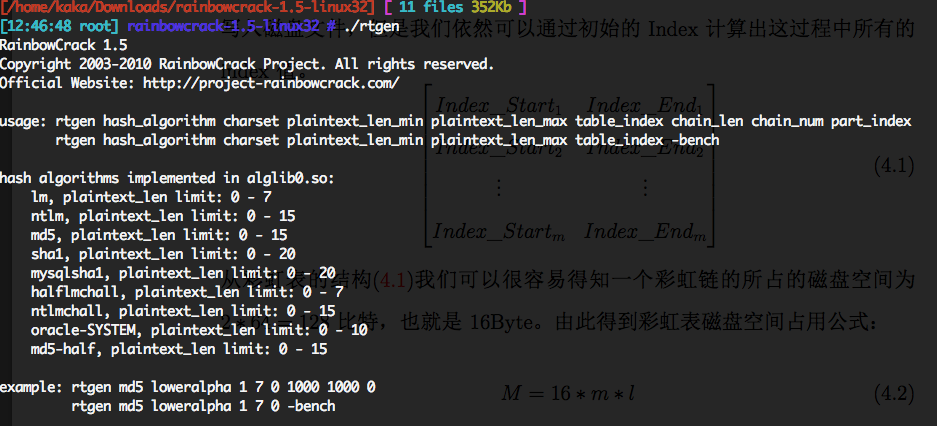
\includegraphics[scale=0.4]{4-1.png}
\caption{彩虹表生成程序}
\label{fig:4.1}
\end{figure}

\begin{figure}[!ht]
\centering
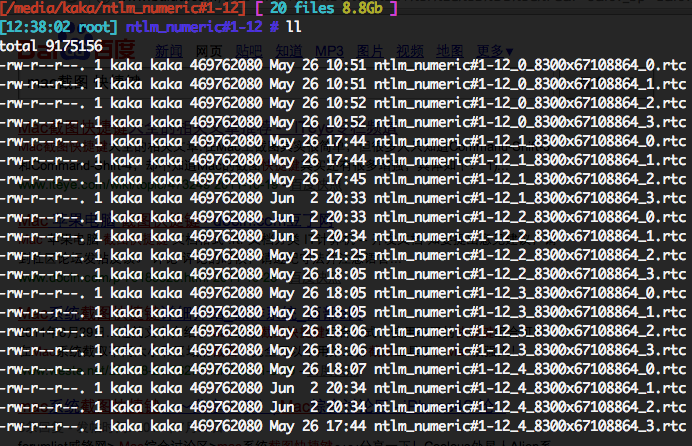
\includegraphics[scale=0.5]{4-2.png}
\caption{ntlm算法彩虹表}
\label{fig:4.2}
\end{figure}
从图\ref{fig:4.2}中我们可以看到20张彩虹表,hash\_algorithm为ntlm算法,ntlm为Windows NT系统的用户登陆验证算法;密钥字符集为numeric,也就是0~9,最小长度为1,最大长度为12,因此这个密钥空间$N=10^{12}+10^{11}+ \cdots +10^2 +10$,其他的密钥并不在这20张表里,一定不会被搜索到,想要破解需要加大链的数目,或者链表长度,或者表的张数;链表长度为8300,链表个数为67108864,这样通过公式\eqref{equ:4.2}我们很容易到这20张表的所占用的磁盘空间$M=20GB$,每张表的大小为1GB。
\section{利用彩虹表进行破解密钥}
\section{本章小结}
